% !TEX root = ../Diplombericht.tex
\subsection{Physikalischer Überblick}
Durch die aufgeführte Abbildung ist eine Übersicht der vorhandenen und angeschlossenen Komponenten des Projektes ersichtlich.

\begin{figure}[htb]
\centering
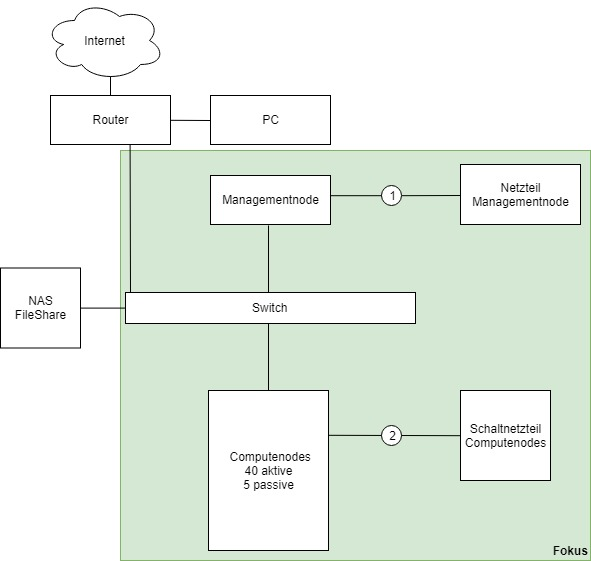
\includegraphics[scale=0.5]{phys_ueberblick.jpg}
\caption{Physikalischer Überblick}
\label{fig:Physikalischer Überblick}
\end{figure} 

\textbf{Beschreibung}\newline
Der grün markierte Teil beinhaltet das Vorhaben. Diese Komponenten werden neu in das Netzwerk eingebunden und aufgebaut. Die Komponenten ausserhalb des grünen Bereiches existieren bereits und es müssen für die Umsetzung Konfigurationen vorgenommen werden.

\textbf{Verbindung 1} \newline
Der Management Node wird über ein herkömmliches Netzteil per Micro USB mit Stom versorgt.

\textbf{Verbindung 2} \newline
Die Compute Nodes werden über ein Schaltnetzteil über die General Purpose Input/Output (GPIO) Pins mit Strom betrieben.


